\section{Results}
\label{sec:results}
We report what each level of the architecture contributes (\cref{fig:framework}): recursive practice (\cref{sec:rq1}), the gate (\cref{sec:rq2}) and the meta level (\cref{sec:rq3}), then how the loop compares with plain RL (\cref{sec:rl}). Every number comes from a preregistered read of a sealed test unless it is marked \emph{gate-level}.

\subsection{Does recursive self-improvement make the policy better?}
\label{sec:rq1}

\begin{table}[t]
  \centering
  \small
  \caption{\textbf{Twelve rounds, two sealed tests} (LIBERO-Goal, cloud pool, seeds 1--3; points, 95\% CI). Official: 500 fixed states, three-evaluation finals. Fresh: 1{,}000 sampled placements, disjoint from every practice, gate and audit set and registered before any evaluation on them.}
  \label{tab:long}
  \resizebox{\linewidth}{!}{%
  \begin{tabular}{@{}lccc@{}}
    \toprule
    comparison & bar & official test & fresh scenes \\
    \midrule
    \texttt{fixed12} $-$ start & $+5$ & $+1.60$ $[-0.88, +4.13]$ & $+3.54$ $[+1.72, +5.42]$ \\
    \texttt{fixed12} $-$ \texttt{nonrec12} & $+2$ & $+7.84$ $[+5.22, +10.49]$ & $+7.30$ $[+5.47, +9.20]$ \\
    \texttt{fixed12} $-$ \texttt{onebig12} & $+2$ & $-0.38$ $[-2.42, +1.64]$ & $-2.73$ $[-4.30, -1.20]$ \\
    \bottomrule
  \end{tabular}}
\end{table}

\textbf{Finding 1: recursive self-practice improves the policy on unseen scenes, and recursion is what makes it work.} A registered twelve-round study (three seeds each of \texttt{fixed12}, \texttt{nonrec12} and a 36-step \texttt{onebig12}) was read on both sealed tests (\cref{tab:long}). On 1{,}000 fresh scenes that no run trained, gated or audited on, the recursive loop ends $+3.5$ points $[+1.7, +5.4]$ above its start, on every seed; the registered bar was $+5$ and is missed. The same loop with practice generated by the frozen initial policy ends $3.8$ points \emph{below} its start, so recursion is worth $+7.3$ $[+5.5, +9.2]$ on the fresh scenes and $+7.8$ $[+5.2, +10.5]$ on the official test, positive on every seed and well over its $+2$ bar on both. The mechanism is visible in the records: once the learner has moved, practice generated by the initial policy no longer matches it, its candidates are truly a little worse than their parent, and with acceptance on $\ge$ noise-driven acceptances accumulate, although every \texttt{nonrec12} version passed a fresh paired gate. Recursive practice keeps the data on the learner's own distribution, which is the point of letting the system generate its own practice.

\begin{table*}[t]
  \centering
  \small
  \caption{\textbf{Registered claims on LIBERO-Goal} (official 500-episode test, 3-evaluation finals, pooled initial reference, seed-averaged paired bootstrap). Platform Y = cloud pool, A = A800.}
  \label{tab:goal}
  \begin{tabular}{@{}llrrcc@{}}
    \toprule
    claim & comparison & points & 95\% CI & bar & seeds \\
    \midrule
    R1 & \texttt{fixed} $-$ ref. (Y) & $+1.71$ & $[-0.76, +4.23]$ & $+5$ & 1--3 \\
    R1 & \texttt{full} $-$ ref. (Y) & $+1.28$ & $[-1.37, +3.99]$ & $+5$ & 1--3 \\
    R2 & \texttt{fixed} $-$ \texttt{shuffled} (Y) & $+1.22$ & $[-0.37, +2.85]$ & $+3$ & 0--3 \\
    R3 & \texttt{fixed} $-$ \texttt{nonrec} (Y) & $+1.72$ & $[-0.28, +3.68]$ & $+2$ & 0--3 \\
    R4 & \texttt{full} $-$ \texttt{fixed} (Y) & $-0.42$ & $[-2.40, +1.56]$ & $+2$ & 1--3 \\
    R4 & \texttt{llm\_harness} $-$ \texttt{fixed} (Y) & $-0.73$ & $[-2.58, +1.07]$ & $+2$ & 1--3 \\
    R4 & \texttt{llm} $-$ \texttt{fixed} (A) & $+1.04$ & $[-0.84, +3.00]$ & $+2$ & 1--3 \\
    R4 & \texttt{llm\_harness\_cap} $-$ \texttt{fixed} (A) & $+1.16$ & $[-0.76, +3.16]$ & $+2$ & 1--3 \\
    R5 & best gated $-$ \texttt{onebig} (Y) & $-0.58$ & $[-2.12, +0.95]$ & $+2$ & 0--3 \\
    \midrule
    noise & half vs.\ half of the n0 evaluations (Y / A) & $+0.64$ / $+0.54$ & $[-0.07, +1.36]$ / $[-0.24, +1.35]$ & & \\
    \bottomrule
  \end{tabular}
\end{table*}

\begin{figure*}[t]
  \centering
  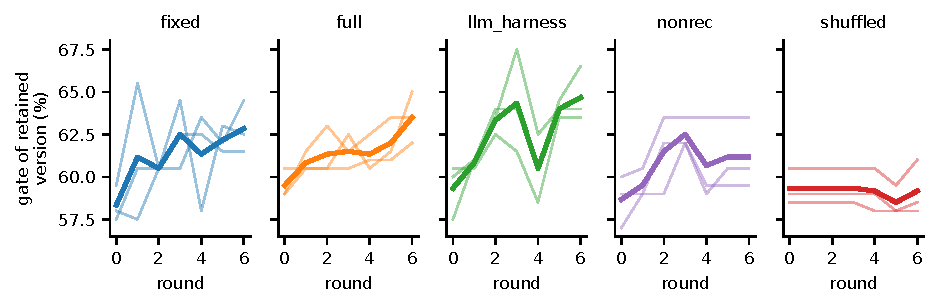
\includegraphics[width=\textwidth]{fig_gates}
  \caption{\textbf{Gate success of the retained policy by round} (cloud platform; thin lines are seeds 1--3, the thick line their mean). A dot marks a round that accepted a new version; every round is scored on 200 newly drawn placements, so a retained version's score can fall from one round to the next. The number in each panel is the change of the mean from round 0 to round 6. With a real verifier and recursive practice the loop climbs 4--5 points at the gate within six rounds; without the verifier (\texttt{shuffled}) it stays flat, and with practice from the frozen initial policy (\texttt{nonrec}) it stops after round 3. Gate gains overstate test gains by the winner's curse (\cref{tab:arms}).}
  \label{fig:gates}
\end{figure*}

\begin{table}[t]
  \centering
  \small
  \caption{\textbf{Per-arm finals} (\%, mean of the 3-evaluation finals over seeds 1--3; seed-0 runs listed separately). Reference 58.9 (Y) / 58.4 (A).}
  \label{tab:arms}
  \resizebox{\linewidth}{!}{%
  \begin{tabular}{@{}lcccccc@{}}
    \toprule
    & \texttt{fixed} & \texttt{full} & \texttt{llm$\ast$} & \texttt{nonrec} & \texttt{shuf.} & \texttt{onebig} \\
    \midrule
    Y, s1--3 & 60.6 & 60.2 & 59.9 & 59.1 & 58.9 & 59.1 \\
    A, s1--3 & 59.1 & -- & 60.1 / 60.2 & -- & -- & -- \\
    A, s0 & 57.2 & -- & -- & 54.8 & 57.5 & 62.7 \\
    \bottomrule
  \end{tabular}}\\[2pt]
  {\footnotesize $\ast$ Y: \texttt{llm\_harness}; A: \texttt{llm} / \texttt{llm\_harness\_cap}.}
\end{table}

\textbf{Finding 2: at six rounds the gains are small, and verified, recursive practice is where they come from.} Every gated run ends within noise of its start or above it (finals 57.1--62.2\% against a reference of 58.4--58.9\%; \cref{tab:arms}); the typical gain is one to two points, the best single seed gains $+3.3$ $[+0.1, +6.6]$, and the registered improvement claim R1 comes to $+1.71$ $[-0.76, +4.23]$ against a $+5$ bar (\cref{tab:goal}). The two largest ingredients are recursion (R3 $+1.72$ $[-0.28, +3.68]$, just under its $+2$ bar) and the verifier (R2 $+1.22$): without a real verifier the loop ends where it started. At the gate (\cref{fig:gates}) the separation is visible within six rounds; at twelve it reaches the sealed tests (Finding 1).

\subsection{Is self-training safe? The gate}
\label{sec:rq2}

\textbf{Finding 3: the gate is what keeps self-training from collapsing.} The behaviour-cloning recipe of \cref{sec:rq3} collapses from 58.5\% to 5.5\% on held-out placements when its versions are accepted unconditionally (\cref{fig:teaser}b); under fresh paired gates the same recipe does not fall below its start beyond noise on the sealed test, and no gated run of the main study does. The gate is cheap (one extra evaluation per candidate) but noisy: a 200-episode paired comparison has a standard deviation of about 3.4 points, so it accepts and rejects many candidates by chance. Its protection relies on recursive practice: over twelve rounds a chain of gate-accepted \texttt{nonrec12} versions drifts below its start (Finding 1).

\subsection{Can the system improve its own training procedure? The meta level}
\label{sec:rq3}

\paragraph{A recipe that fails.} The meta level can be told apart from RL only where RL's recipe fails. One such case was found before any meta-level run: behaviour cloning on the policy's own temperature-1.6 samples with a unit-temperature likelihood collapses when its versions are accepted unconditionally. The repair is a one-knob change (the BC temperature, the sampling temperature or the update operator), and all three knobs are in the harness space, but the meta level is never told which. A registered study starts from this recipe with arms \texttt{fixed} (the gate alone), \texttt{full} (numeric search) and \texttt{llm\_harness} (same compute), four seeds, and the bar S1 $=$ \texttt{llm\_harness} $-$ \texttt{fixed} $\ge +3$, CI above 0.

\begin{figure*}[t]
  \centering
  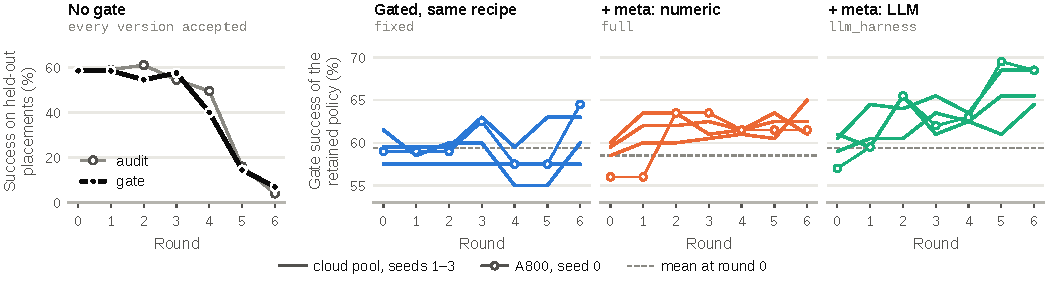
\includegraphics[width=\textwidth]{fig_selfrepair}
  \caption{\textbf{Self-repair study, gate level.} Left: the starting BC recipe collapses when every version is accepted. Right (narrower scale): under the gate the same recipe stays at its starting level (\texttt{fixed}); both proposers find repairs; at the gate the LLM arm looks 4--8 points ahead, on the sealed test it is $+2.65$ (\cref{tab:selfrepair}).}
  \label{fig:selfrepair}
\end{figure*}

\begin{table}[t]
  \centering
  \small
  \caption{\textbf{Self-repair study}: gate / sealed-test final (\%, three evaluations) of each retained version, and what changed. S1 $=$ \texttt{llm\_harness} $-$ \texttt{fixed} $= +2.65$ $[+0.73, +4.58]$ (bar $+3$ missed); S2 $=$ \texttt{llm\_harness} $-$ \texttt{full} $= +1.15$ $[-0.63, +2.92]$; S3 $=$ \texttt{llm\_harness} $-$ hand-tuned GRPO loop $= +0.28$ $[-1.43, +1.97]$.}
  \label{tab:selfrepair}
  \resizebox{\linewidth}{!}{%
  \begin{tabular}{@{}llll@{}}
    \toprule
    seed & \texttt{fixed} (gate only) & \texttt{full} (numeric) & \texttt{llm\_harness} \\
    \midrule
    1 (Y) & 60.0 / 56.1 & 62.5 / 56.7 & 65.5 / 60.1, GRPO in r1 \\
    2 (Y) & start / 58.7, all refused & 65.0 / 59.9, GRPO & 68.5 / 61.3, GRPO in r1 \\
    3 (Y) & 63.0 / 57.5 & 61.0 / 60.2, BC rollout-$T$ & 64.5 / 57.9, BC $T$ 1.6$\to$1.3 \\
    0 (A) & 64.5 / 57.4 & 61.5 / 58.8 & 68.5 / 60.9, GRPO in r2 \\
    \bottomrule
  \end{tabular}}
\end{table}

\textbf{Finding 4: the meta level diagnoses and repairs a failing training procedure on its own.} On all four seeds the language model's first-round diagnosis names the mismatch between the sampling and likelihood temperatures and the missing failure signal (verbatim in the released logs), and its first proposal is the same: switch to GRPO on mixed-outcome scenes at a lower temperature. The gate kept that switch in round 1--2 on three seeds and refused it twice on the fourth, where the model repaired BC instead (\cref{tab:selfrepair}). The repaired loop then gains what the hand-tuned loop gains: S1 $= +2.65$ points $[+0.73, +4.58]$ over the gate alone, positive on three seeds with the interval above zero, and level with the hand-tuned GRPO loop (S3 $= +0.28$ $[-1.43, +1.97]$), while the gate alone holds the policy at its start ($-2.37$ $[-4.12, -0.62]$ against the hand-tuned loop). Two qualifications are registered. S1 is under its $+3$ bar, so the claim is not made in its registered form. And numeric search over the same knobs also finds a repair, on two seeds and only in round 6, ending $1.15$ points behind ($[-0.63, +2.92]$): the model's advantage is speed and reliability of the diagnosis, not a better end point. Six gate-only pilots with extreme GRPO and BC recipes found no second failing scenario.

\textbf{Finding 5: on a recipe that already works, the meta level finds nothing to repair.} All four meta-level arms of the main study land within $\pm 1.2$ points of \texttt{fixed} (R4, \cref{tab:goal}). A second registered study (``v2'') gives the model per-task gate rates with their noise and compares it with a \emph{replica} arm that trains the identical recipe at the same compute: $-0.27$ $[-2.53, +2.00]$ (cloud, seeds 1--3) and $+0.30$ $[-1.60, +2.15]$ (A800, seeds 0--3). The records show why. The model's diagnoses are correct (an unsolved task gives GRPO no signal, another is saturated, the remaining gate changes are noise) and its edits are those a practitioner would try, but its proposals scored $-1.2$ points against the incumbent at the gate ($n{=}30$) where replicas scored $+0.6$ (sd 3.4, $n{=}36$): \emph{every recipe in the space reaches the same plateau}, so there is nothing for a correct diagnosis to fix.

\subsection{Against plain RL at equal compute}
\label{sec:rl}

\textbf{Finding 6: a strictly gated loop does not beat plain RL on a recipe that works.} One round of plain RL with the whole budget (\texttt{onebig}) matches the six-round loop (R5 $-0.58$ $[-2.12, +0.95]$), ties the twelve-round loop on the official test ($-0.38$) and is $2.7$ points ahead of it on the fresh scenes (\cref{tab:long}). The cost is the gate's strictness: the twelve-round runs kept 6, 9 and 9 of their 12 rounds, a refused round's training is discarded, and most refusals in our records are dips within the gate's own noise. Training without a gate loses no rounds, but has no protection either: without it the BC recipe of \cref{fig:teaser}b collapses.

\subsection{How much of a published VLA-RL number is the test set?}
\label{sec:rq4}

\begin{figure}[t]
  \centering
  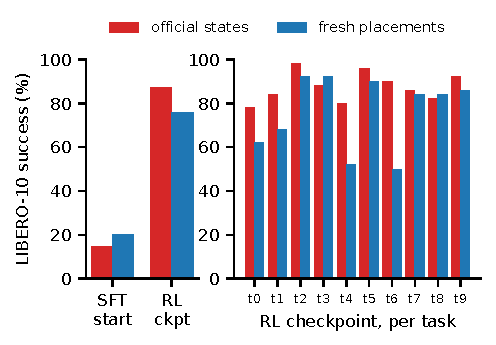
\includegraphics[width=\linewidth]{fig_inflation}
  \caption{\textbf{Train-on-test inflation} (LIBERO-10). Left: official vs.\ fresh placements for the SFT start and the RL checkpoint trained on the official states. Right: the RL checkpoint per task; the loss is concentrated on tasks 4 and 6.}
  \label{fig:inflation}
\end{figure}

\textbf{Finding 7: about a fifth of the headline number.} The released SimpleVLA-RL LIBERO-10 checkpoint was trained by RL on the 50 fixed test states per task. We evaluated it, and its own SFT start, on the 500 official episodes and on 500 placements freshly drawn by LIBERO's own sampler (the same distribution, not a perturbation): SFT 14.6\% official against 20.0\% fresh, RL 87.4\% against 76.0\%. The difference of the two gaps, which cancels any difference in difficulty between the placement sets, is $+16.8$ points $[+9.8, +23.4]$; 500 further never-seen placements give $+16.0$ $[+9.2, +22.4]$ (\cref{fig:inflation}). The method works (the checkpoint gains 56 points on fresh placements), but about a fifth of its headline number is memorisation of the test states.
